\section{A Dinâmica de Formas}\label{secao:dinamica_de_formas}
A Dinâmica de Formas (SD, do inglês \textit{Shape Dynamics}) é uma teoria de gravitação baseada em \textit{relacionalismo}, isto é, os conceitos absolutos de \textit{espaço} e de \textit{tempo} são suprimidos para basear a física na relação entre os objetos em questão - no caso do PNCG, a relação entre os corpos.

Embora seja um modelo alternativo de gravitação, foi a partir dela que começamos o estudo do PNCG como um todo, através do artigo \cite{Barbour2014_identification}. Por isso, apresentamos nesta seção uma breve introdução à versão quantizada (em massas pontuais) da SD e alguns de seus resultados qualitativos, que na seção \ref{secao:simulacao_dinamica_de_formas} são revisitados e podem ser visualizados através de simulações numéricas.

Nesta seção, algumas demonstrações foram omitidas tendo em vista facilitar a leitura do texto. Estas se encontram no Apêndice \ref{apendice:demonstracoes_dinamica_de_formas}. Além disso, as referências utilizadas encontram-se citadas no texto, mas as principais são o artigo mencionado, \cite{barbour2013_gravitationaloriginarrowstime} e \cite{Barbour2014_solution}.

%%%%%%%%%%%%%%%%%%%%%%%%%%%%%%%%%%%%%%%%%
\subsection{Contextualização e motivação}

O objetivo da Dinâmica de Formas é fornecer um modelo de gravitação que comporte a compreensão mecânica do físico e filósofo Ernst Mach (1838-1916), na qual apenas as relações inter-partícula são \textit{reais}. Para o problema de N-corpos em $\R^{3N}$, tomamos o quociente pelas translações e rotações euclidianas, obtendo o \textit{espaço de configurações relativas} (ECR) machiano, de $3N-6$ dimensões, o que remove as posições e orientações absolutas. Mais ainda, é preciso quocientar o ECR também em relação a \textit{dilatações}, para remover qualquer influência de escalas. Nisso, obtemos o \textit{espaço de formas} $S$ com $3N-7$ dimensões. 

Observe que ao quocientar $\R^{3N}$ pelas translações, a mecânica vigente ainda é a mecânica newtoniana, uma vez que o potencial newtoniano é invariante sob translações. Já para rotações, a situação não é a mesma, sendo o momento angular um elemento crucial de subsistemas fechados do universo (como o Sistema Solar). O modelo, então, se baseia no pressuposto de que não há rotação global no universo, mas somente rotações locais de subsistemas \citep[264]{Barbour2012_sd_introduction}.

Nessa situação, se torna aplicável um princípio que, embora não tenha sido enunciado diretamente por Mach, decorre de sua filosofia \citep[139]{Assis:1998}, que é chamado de \textit{princípio de Mach} ou \textit{de Mach-Poincaré}:

\begin{definition}[Princípio de Mach-Poincaré]
    A especificação de um ponto e uma direção (\textbf{forma forte}) ou de um ponto e um vetor tangente (\textbf{forma fraca}) no espaço de formas $S$ determinam a evolução em $S$ de forma única. \citep[31]{Barbour2014_kepler_mach}
\end{definition}

É fato importante que como um modelo de gravidade aplicável, existe uma interseção entre a Dinâmica de Formas e a Relatividade Geral, ocorrendo quando a Relatividade Geral comporta o Princípio de Mach-Poincaré: universos espacialmente fechados (\citealp[157]{Einstein:1981}; \citealp[258]{Barbour2012_sd_introduction}).

De toda forma, há diversas consequências da SD que são interessantes para a física, desde o próprio modelo de gravitação até implicações para uma gravidade quântica \citep{Barbour2012_sd_introduction}. Para este trabalho, o que interessa é a formulação de setas do tempo relacionais, uma forma de observar a evolução de sistemas de N-corpos baseada somente no próprio sistema.

%%%%%%%%%%%%%%%%%%%%%%%%%%%%%%%
% PRIMEIRO, PRECISO FALAR DO POR QUE QUERER SETAS DO TEMPO
% - MUITOS QUEREM DESCREVER A EVOLUÇÃO UTILIZANDO A ENTROPIA. O CONCEITO ORIGINAL NÃO FAZ SENTIDO PARA O PNCG, POIS A GRAVIDADE É DOMINANTE, O UNIVERSO NÃO TEM PAREDES E UM VOLUME GLOBAL FAZ ENTENDER QUE EXISTE ALGO MAIOR PARA REFERENCIAR.
Uma seta do tempo é um observável que não apenas caracteriza a evolução de um sistema dinâmico, mas também fornece uma orientação, no sentido de determinar o que é \textit{passado} e o que é \textit{futuro}. Na física, a maioria das discussões de setas do tempo se baseia no crescimento da entropia, uma medida de ``dispersibilidade'' de um sistema. Porém, no caso de sistemas puramente gravitacionais e fechados, a entropia como seta do tempo é uma escolha bastante questionável por algumas razões. Por exemplo, a conceitualização original de entropia se baseia em partículas fechadas em um espaço confinado e em um volume total do espaço de fases; ambas as bases não se encaixam ao Universo enquanto um sistema máximo no qual a gravidade é a força dominante.

% - A IDEIA ENTÃO É ABSTRAIR TODAS AS ESTRUTURAS EXTERNAS DA DINÂMICA DO PROBLEMA. NO PNCG, SÃO A POSIÇÃO, ORIENTAÇÃO E TAMANHO EM UM REFERENCIAL INERCIAL E UM TEMPO EXTERNO. UMA HISTÓRIA DINÂMICA É UMA CURVA UNPARAMETRIZED EM S. AS EQUAÇÕES DE MOVIMENTO DO PNCG SÃO SIMETRICAS NO TEMPO, ENTÃO NÃO DEFINEM UMA ORIENTAÇÃO EM C. TAMBEM POR ISSO, ENTROPIA E OUTRAS SETAS NÃO FAZEM SENTIDO.

% - UMA SETA DIGNA ENTÃO PRECISA TER ORIGEM EM UMA ASSIMETRIA DENTRO DO ESPAÇO S

Voltando ao enunciado sobre o princípio de Mach, o que realmente caracteriza a dinâmica do PNCG está no espaço $S$. Porém, as equações de movimento de Newton são simétricas no tempo, e portanto incapazes de fornecer uma orientação para a evolução de uma órbita em $S$. Assim, uma seta do tempo para o PNCG precisa ser caracterizada por alguma assimetria dentro do próprio espaço de formas.

% - COMO A ESCALA (DEGREES OF FREDOM) É UNICA E TEM DIMENSÕES, DEPENDENDO DE UMA ESCALA EXTERNA DEFINIDA, É PRECISO QUE AS SHAPE DOF NÃO TENHAM ESSE PROBLEMA. ATRAVÉS DE UMA DEPARAMETRIZAÇÃO, TRANSFORMAMOS A VARIÁVEL DE ESCALA (R) EM UM HAMILTONIANO (LOG R) E O SEU MOMENTO CONJUGADO MONÓTONO (D) NO PARÂMETRO DE EVOLUÇÃO (t). RESTA O MENOR CONJUNTO DE VARIÁVEIS NECESSÁRIAS PARA DESCREVER O UNIVERSO OBJETIVAMENTE.

\subsection{Eliminação da escala}
Uma questão sobre o PNCG é que o sistema comporta escalas. No entanto, já foi apresentado que através do Teorema \ref{teorema:similaridade_dinamica} é possível ignorar a escala, uma vez que aplicar um redimensionamento anisotrópico sobre uma trajetória fornece um conjunto de trajetórias com dinâmicas iguais a menos da escala. Uma representação objetiva do problema precisa ser capaz de condensar esse conjunto infinito de trajetórias dinamicamente equivalentes em uma única órbita em $S$. 

Para isso, podemos utilizar a raiz quadrada do momento de inércia $R$, pois este representa um tipo de \textit{desvio padrão} do sistema. Nesse caso, é preciso balancear cada posição com relação a sua massa, aplicando a transformação:
\begin{equation}
    \vet \sigma_a = \dfrac{\sqrt{m_a}}{R} \vet q_a,
    \quad a = 1, 2, ..., N.
\end{equation}
Observe que $\vet \sigma_a$ é adimensional. Além disso, trata-se uma coordenada dentro de uma bola unitária espacial na origem de $S$, uma vez que, por exemplo, para $N=1$ tem-se:
\begin{equation*}
    \vet \sigma_a = \dfrac{\sqrt{m_a} \vet q_a}{\sqrt{m_a} \norma{\vet q_a}} = \dfrac{\vet q_a}{\norma{\vet q_a}},
\end{equation*}
e valores maiores de $N$ oferecem um denominador maior que o numerador.

Podemos obter momentos conjugados para as coordenadas $\vet \sigma_a$ e que atendem à expectativa relacional, de que só é possível estar em movimento se for em relação a outra partícula:
\begin{equation*}
    \vet \pi_a = \dfrac{R}{\sqrt{m_a} D_0} \vet p_a - \dfrac{D}{D_0} \vet \sigma_a, \quad \forall a = 1, ..., N,
\end{equation*}
onde $D$ é o momento de dilatação ($D = R \dot R $). De fato, um sistema de uma só partícula não tem movimento:
\begin{equation*}
    \vet \pi_a 
    = \dfrac{\sqrt{m_a} \norma{\vet q_a}}{\sqrt{m_a} D_0} \vet p_a - \vet q_a \cdot \vet p_a \dfrac{\vet q_a}{D_0 \norma{\vet q_a}}
    = \dfrac{1}{D_0} (\norma{\vet q_a} \vet p_a - \vet p_a \norma{\vet q_a}) 
    = \vet 0, \quad \text{ se } N = 1.
\end{equation*}
Vale ressaltar que o par de coordenadas projetadas $(\vet \sigma, \vet \pi)$ (chamadas a partir daqui de \textit{objetivas}) ainda não é invariante por rotações. No entanto, obter uma forma explícita e rotacionalmente invariante é difícil, além de pouco produtivo, uma vez que o momento angular comuta em Poisson com a função hamiltoniana. (\citealp[21]{barbour2013_gravitationaloriginarrowstime}; \citealp{Barbour2014_identification}). Além disso, como esperado, as coordenadas objetivas possuem propriedades que correspondem às invariâncias exigidas por uma dinâmica adimensional:
\begin{align}\label{eq:new_constraints}
    R_{\vet \sigma} = \sum_{a=1}^N \vet \sigma_a \cdot \vet \sigma_a = 1, \quad
    D_{\vet \sigma, \vet \pi} = \sum_{a=1}^N \vet \pi^a \cdot \vet \sigma_a = 0, \nonumber \\
    \vet \sigma_{cm} = \sum_{a=1}^N \sqrt{m_a} \vet \sigma_a = 0, \quad
    \vet \pi_{\Sigma} = \sum_{a=1}^N \sqrt{m_a} \vet \pi^a = 0.
\end{align}
A restrição $R_{\vet \sigma}$ força que o sistema seja unitário, pois o que está se fazendo na prática é normalizar $R$. A restrição $D_{\vet \sigma, \vet \pi}$ corresponde ao processo para $D$, representando a invariância da escala global. Já $\vet \sigma_{cm}$ corresponde à ausência de movimento do sistema como um todo, análogo à conservação do centro de massas. Por fim, $\vet \pi_{\Sigma}$ corresponde à invariância do momento total. A demonstração destas propriedades consta no Apêndice \ref{apendice:demonstracoes_dinamica_de_formas} (Proposição \ref{prop:new_constraints}).

Também é possível verificar que $(\vet \sigma, \vet \pi)$ são invariantes por escala, uma vez que comutam com $D$ e com $R$ no sistema de coordenadas original
\begin{equation}\label{eq:invariancia_por_escala}
    \{ f(D,R), \vet \pi_a \} = \{ f(D, R), \vet \sigma_a \} = 0,
\end{equation}
onde $f$ é um observável para $D$ e $R$ (Proposição \ref{prop:invariancia_por_escala})

% - COMO SABER QUE SAO R E D? PRECISO ENUNCIAR NOVAMENTE O MOMENTO DE INERCIA, R E D E ATRAVES DE LAGRANGE-JACOBI MOSTRAR QUE D É MONÓTONO. USANDO O PARENTESE DE POISSON, POSSO MOSTRAR QUE O D É O MOMENTO CONJUGADO MONOTONO DE LOG R, ENTÃO FAZ SENTIDO FAZER

\subsection{Evolução de um sistema adimensional e complexidade}
Uma vez que o sistema deixa de ter escala, sua evolução depende de um correspondente à evolução da escala no problema original. Nesse caso, o momento de dilatação $D$ pode ser interpretado como variável de evolução para $E \geq 0$, uma vez que $D$ é monótono (Teorema \ref{teorema:lagrange_jacobi}). Para descrever o sistema nessa situação, é necessário um hamiltoniano baseado em $R$ e com variável baseada em $D$ que gere translações. Para isso, embora $R$ não seja canonicamente conjugado a $D$, $\log R$ é (veja equação \ref{eq:poisson_coordenadas_canonicas}), pois
\begin{equation*}
    \{\log R, D \} 
    = \sum_{a=1}^{N} \derpar{\log R}{\vet q_a} \derpar{D}{\vet p_a} - \derpar{\log R}{\vet p_a} \derpar{D}{\vet q_a}
    = \sum_{a=1}^{N} \dfrac{1}{R^2} m_a \norma{\vet q_a}^2 
    = 1.
\end{equation*}
Dessa forma, tomando uma variável de tempo adimensional $\tau = D/D_0$ (considerando $D_0 \neq 0$), temos um hamiltoniano $\mathcal H = - \log{(R/R_0)} + const$.

Descrever a energia cinética desse novo sistema não é difícil. Podemos decompor a energia cinética original em duas partes, uma correspondente à \textit{dilatação} $T_d = \frac{1}{2} D^2 / R^2$ e outra correspondente à \textit{forma} $T_S = \frac{1}{2} D_0^2 K_S / R^2$, onde
\begin{equation*}
    K_S = \sum_{a=1}^{N} \vet \pi_a \cdot \vet \pi_a = \dfrac{2 R^2 T - D^2}{D_0^2},
\end{equation*}
pois
\begin{equation*}
    T_d + T_S
    = \dfrac{1}{2} \dfrac{D^2}{R^2} + \dfrac{D_0^2}{2 R^2} K_S
    = \dfrac{1}{2} \left( \dfrac{D^2}{R^2} + 2 T - \dfrac{D^2}{R^2} \right) = T.
\end{equation*}

% - MAS COMO VAMOS DESCREVER A DINAMICA AQUI? PRECISAMOS DE UMA FUNÇÃO POTENCIAL PRA COISA, E ELA PRECISA SER 1/r² PARA QUE {H, D} = 0. O QUE CARACTERIZA BEM A EVOLUÇÃO DO SISTEMA? BOM, TEMOS OS TAMANHOS: L_RMS (R/M) E L_MHL (-V/M). A RAZAO DISSO FORNECE UMA MEDIDA DE COMPLEXIDADE BEM LEGAL QUE É INTRINSECA EM S.

A energia potencial, por outro lado, exige mais atenção. Como queremos um sistema invariante por escala, precisamos que o potencial seja homogêneo de grau $-2$ \citep[5]{Barbour2013_scaleanomaly}. Por outro lado, observando o sistema original, há duas medidas que caracterizam a dinâmica entre os corpos: a \textit{raiz da média quadrática} $\ell_{rms}$:
\begin{equation*}
    \ell_{rms} := \dfrac{1}{M^{1/2}} R,
\end{equation*}
e o \textit{comprimento harmônico médio} $\ell_{mhl}$:
\begin{equation}
    \ell_{mhl} = \dfrac{M^2}{|V|}.
\end{equation}
O comprimento $\ell_{rms}$ é uma medida interessante para o sistema como um todo, uma vez que dominam as maiores distâncias entre os corpos. Por outro lado, $\ell_{mhl}$ é uma medida bastante caracterizada pelas menores distâncias entre os corpos, uma vez que é inversamente proporcional às distâncias.

Unindo a necessidade de um potencial com grau $-2$ com o que se sabe sobre as escalas, podemos definir a complexidade
\begin{equation}
    C_S := \dfrac{\ell_{rms}}{\ell_{mhl}} = \dfrac{1}{M^{3/2}} R |V|.
\end{equation}
Observe que, além de atender o desejado, também trata-se de uma medida adimensional, sendo portanto \textit{intrínseca} do espaço $S$.

\begin{figure}
    \centering
    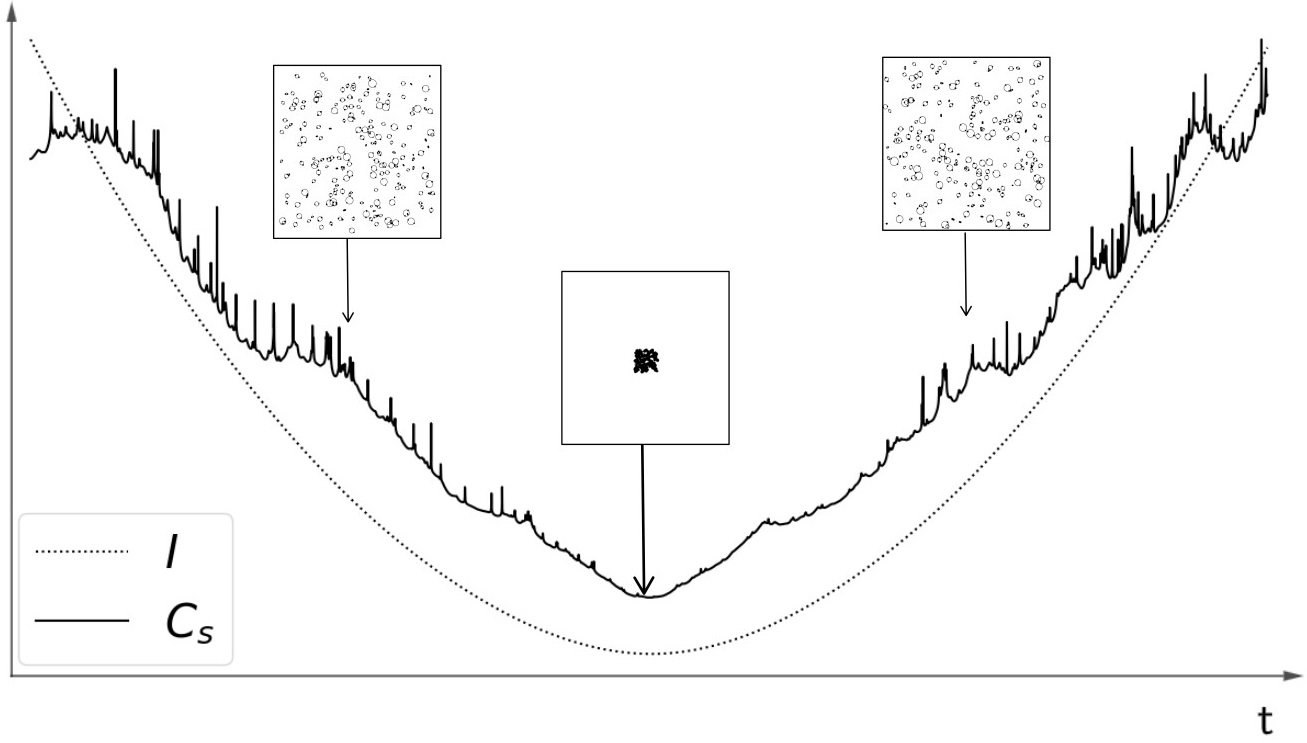
\includegraphics[width=0.5\linewidth]{tcc//img/complexidade.jpg}
    \caption{Visualização do espalhamento. O gráfico da complexidade corresponde a uma simulação de 100 corpos para $E=0$.}
    \label{fig:exemplo_espalhamento}
\end{figure}

% - A C_S É BOA POR DIVERSAS RAZÕES. ELA CARACTERIZA BEM TANTO A EVOLUÇÃO GERAL DO SISTEMA QUANTO O COMPORTAMENTO EM PEQUENA ESCALA. ELA CRESCER VARIANDO SIGNIFICA QUE A DISTANCIA ENTRE OS CORPOS FICA OSCILANDO.

% - SEGUNDO SAARI, PARA E = J = 0 O SISTEMA EVAPORA EM SUBSISTEMAS E CADA SUBSTISTEMA COMEÇA A CONVERGIR NO GERAL PARA CONSTANTES DE MOVIMENTO. QUANTO MAIS DIGITOS SAO CONSERVADOS EM UM SUBSISTEMA, MAIS ELE ESTÁ DISTANTE NA EVOLUÇÃO, ENTÃO A COMPLEXIDADE CARACTERIZA ISSO, A COMPLEXIDADE DO SISTEMA, O QUÃO ELE ESTÁ COMPLEXO. 

No caso em que $E=0$ e $\vet J = \vet 0$, \cite{Marchal1976} mostra que o sistema se divide em subsistemas (indexados por $\mathcal J$), e que cada subsistema, na medida em que se isola cada vez mais, desenvolve quantidade assintoticamente conservadas:
\begin{align*}
    E_{\mathcal J} (t) &= E_{\mathcal J} (\infty) + O(t^{-5/3}),\\
    \vet J_{\mathcal J} (t) &= \vet J_{\mathcal J} (\infty) + O(t^{-2/3}),\\
    \vet X_{\mathcal J} (t) / t &= \vet V_{\mathcal J} (\infty) + O(t^{-1/3}),
\end{align*}
onde $\vet X_{\mathcal J}$ é a distância do subsistema $\mathcal J$ ao centro de massas total do sistema e $\vet V_{\mathcal J} (\infty)$ é uma constante para a qual $\vet X_{\mathcal J}/t$ tende assintoticamente. Nessa situação, a complexidade caracteriza não apenas o distanciamento total entre os corpos, mas também as variações dentro dos subsistemas, como pode ser observado na figura \ref{fig:exemplo_espalhamento}, na qual $C_S$ cresce (indicando expansão do sistema) mas também varia (indicando as oscilações nos subsistemas).

% - ALEM DISSO, C_S É UM POTENCIAL DA FORMA DESEJADA, E UMA VEZ QUE R REMOVE A DEPENDENCIA DE ESCALA DE V_NEW, AS FORÇAS DERIVADAS DE C_S PODEM APENAS MUDAR A FORMA (SHAPE) DO SISTEMA, E NÃO O SEU TAMANHO. - LOG C_S TOMA O PAPEL DE POTENCIAL QUE ATRAI O SISTEMA TOWARDS MORE INHOMOGENEOUS SHAPES, E TEM MINIMOS E PONTOS DE SELA, MAS NAO MAXIMO GLOBAL.

\subsection{Equações de movimento no espaço de formas $S$}

Outro ponto para a complexidade como energia potencial do sistema é o fato de que $R$ remove a dependência da escala de $V$, então as forças derivadas de $C_S$ são capazes apenas de mudar a forma do sistema, e não o seu tamanho. A função $-\log C_S$ toma o papel de um potencial que leva o sistema para formas mais não-homogêneas.

% - COM ISSO EM MÃOS, AGORA DEFINIMOS AS NOVAS COORDENADAS E PODEMOS RE-ESCREVER O LOG R E OBTER UM HAMILTONIANO LEGAL MAS tau-DEPENDENTE. 

Com a decomposição da energia cinética e a nova energia potencial, agora é possível obter uma expressão para $\mathcal H$ em função de $\vet \sigma$ e $\vet \pi$. Isso é feito tomando em conta que
\begin{equation*}
    R^2 E - M^3 R C_S - \frac{1}{2} D^2 - \frac{1}{2} D_0^2 K_S = 0,
\end{equation*}
e então se $E = 0$ é possível obter uma expressão para $R$, e consequentemente para $\mathcal H$:
\begin{equation}\label{eq:hamiltoniano_tau_dependente}
    \mathcal H (\tau) = \log{(K_S + \tau^2)} - \log{C_S}.
\end{equation}

Para esse hamiltoniano $\tau$-dependente, obtemos um conjunto de equações de Hamilton também $\tau$-dependentes:
\begin{equation}
    \der{\vet \sigma_a}{\tau} = \dfrac{2 \vet \pi_a}{K_S + \tau^2},
    \quad
    \der{\vet \pi_a}{\tau} = \derpar{\log C_S}{\vet \sigma_a} - \dfrac{K_S}{K_S + \tau^2} \vet \sigma.
\end{equation}

% - PODEMOS ENTÃO INTRODUZIR LAMBDA = LOG TAU E DIVIDIR PI POR D, OQ FORNECE UM HAMILTONIANO AUTONOMO QUE DESCREVE METADE DO SISTEMA. POREM, AS EQUAÇÕES AGORA POSSUEM UMA FRICÇÃO NÃO CANONICA -OMEGA QUE ESPONTANEAMENTE DISSIPA O MOMENTO ADIMENSIONAL. ISSO JUNTO DO FATO DO POTENCIAL -LOGCS NAO TER MINIMO LOCAL EXPLICA POR QUE CS CRESCE SECULARMENTE (PORQUE É O OPOSTO DE UM POTENCIAL DE UM SISTEMA COM FRICÇÃO)
\subsection{A escala como fricção em $S$}

A dependência temporal de $\mathcal H$ pode ser eliminada através de uma mudança de coordenadas. Tomando $\lambda = \log \tau$ e definindo $\vet \omega_a = \vet \pi^a / \tau$ como um novo momento conjugado adimensional, obtemos um novo hamiltoniano $H_0$ dado por
\begin{equation}
    H_0 = \log\left(\sum_{a=1}^{N} \vet \omega^a \cdot \vet \omega^a + 1\right) - \log C_s,
\end{equation}
O custo dessa transformação é obter um conjunto não canônico de equações de movimento:
\begin{equation}
    \der{\vet \sigma_a}{\lambda} = \derpar{H_0}{\vet \omega_a},
    \quad
    \der{\vet \omega_a}{\lambda} = - \derpar{H_0}{\vet \sigma_a} - \vet \omega_a.
\end{equation}

O termo $\vet \omega_a$ na equação do momento é um tipo de  \textit{fricção sobre as equações}, indicando que existe dissipação. Dinamicamente, isso indica que o distanciamento dos subsistemas, refletido no problema original no aumento da escala, é refletido em $S$ por uma desaceleração na medida em que se aproxima do bordo da esfera unitária, ao ponto de, no limite, ter velocidade nula. Isso caracteriza uma assimetria sobre as trajetórias em $S$.

Por outro lado, o sistema com $H_0$ indica mais nitidamente o comportamento do sistema. Uma vez que o movimento é regido por um potencial $-\log C_S$ sujeito a fricção linear, $C_S$ deve crescer indefinidamente no problema com integrais primeiras nulas. Além disso, a dinâmica para $H_0$ tem um início delimitado, com um passado distante sendo o ponto-limite em que $D=0$. Isso reforça que $C_S$ possui um mínimo global, denominado \textit{Ponto de Janus}, a partir do qual o sistema pode evoluir em duas direções ($D > 0$ e $D < 0$), sendo cada direção orientada pelo crescimento de $C_S$. Dessa forma, $C_S$ caracteriza uma seta do tempo para o PNCG.

% - SETAS. DESCREVEMOS O PNCG COMO UM SISTEMA DINAMICO NO ESPAÇO DE FORMAS CUJO MOVIMENTO É REGIDO POR UM POTENCIAL -LOG CS SUJEITO A FRICÇÃO LINEAR. NESSE CASO, TEMOS UMA ORIENTAÇÃO PARA O SISTEMA: A DIREÇÃO EM QUE A ESTRUTURA, MEDIDA POR CS, CRESCE.
\subsection{Observações}

O caso em que $\vet J = 0$ mas $E > 0$, porém, é particularmente interessante, pois grande parte da teoria apresentada permanece válida. No lugar do $\mathcal H$ de \ref{eq:hamiltoniano_tau_dependente}, obtemos um hamiltoniano diferente:
\begin{equation*}
    \mathcal H = \log{\left[ C_S + \sqrt{C_S^2 + \frac{1}{2} \epsilon (K_S + \tau ^2)} \right]},
    \quad
    \epsilon = E D_0^2.
\end{equation*}
Nesse caso, o princípio de Mach-Poincaré falha, uma vez que é necessário especificar $\epsilon \tau^2$, mas a dinâmica continua invariante por escala e totalmente adimensional com uma variável monótona independente. No entanto, a evolução final fica mais firmemente estabelecida: o potencial é dependente do tempo e é idêntico a $C_S$ somente no instante inicial, apresentando um comportamento dissipativo com o tempo. Assintoticamente, o sistema congela.

% - QUESTÕES. AS EQUAÇÕES OBJETIVAS EM S MUDAM SE E E J NAO SAO NULOS. NESSE CASO O UNIVERSO CORRESPONDE NÃO APENAS A S MAS A ESTRUTURAS EXTERNAS. POREM, O CASO E = J = 0 BATE COM A ESTRUTURA BÁSICA DO CLOSED-SPACE VACUUM GR E PROVIDENCIA UM MODELO OK PRO UNIVERSO. ALEM DISSO, CS PODE PARECER UM CASAMENTO ARTIFICIAL SÓ PARA DAR ALGO ADIMENSIONAL, MAS O QUE É ARTIFICIAL É SEPARAR R DE V_NEW.
Outros valores para as integrais primeiras podem ser considerados. No entanto, se $E$ e $\vet J$ não são nulos as trajetórias não se resumem a $S$, mas dependem de outras estruturas externas. Uma vez que, como mencionado, o caso com integrais primeiras nulas quando estendido para a versão relativística da Dinâmica de Formas coincide com a Relatividade Geral, são valores razoáveis para se assumir como hipótese.

Outro ponto é sobre o processo de obtenção de $C_S$. Embora soe artificial a definição da complexidade como feita, $C_S$ é adimensional e caracteriza intrinsecamente a dinâmica do PNCG, sendo portanto um valor que de fato \textit{existe} para o problema. Por outro lado, separar a evolução do sistema entre $R$ e $V$, entre os corpos distantes e os corpos próximos, é o que se poderia chamar de artificial.

Assim, para além de um modelo interessante, a Dinâmica de Formas foi introduzida neste trabalho primeiro como motivação, e segundo como uma fonte de propriedades qualitativas do PNCG que podem ser visualizadas através de simulações numéricas. Na seção \ref{secao:simulacao_dinamica_de_formas} nós retomamos e aplicamos numericamente um pouco do que foi apresentado nesta seção.


% Nesse sentido, para $E \geq 0$, como $D$ é monótono este pode ser usado como uma medida de tempo $\tau = D/D_0$, onde $D_0 = D(t_0)$.

% \begin{figure}
%     \centering
%     \includegraphics[width=0.5\linewidth]{tcc//img/complexidade1000.png}
%     \caption{N=1000, h=0.04, e=0.04, [-10³, 10³], verlet, 464s + 451s}
%     \label{fig:enter-label}
% \end{figure}
% \begin{figure}
%     \centering
%     \includegraphics[width=0.5\linewidth]{tcc//img/complexidade_1000_energia_0.png}
%     \caption{Enter Caption}
%     \label{fig:enter-label}
% \end{figure}

% \begin{figure}
%     \centering
%     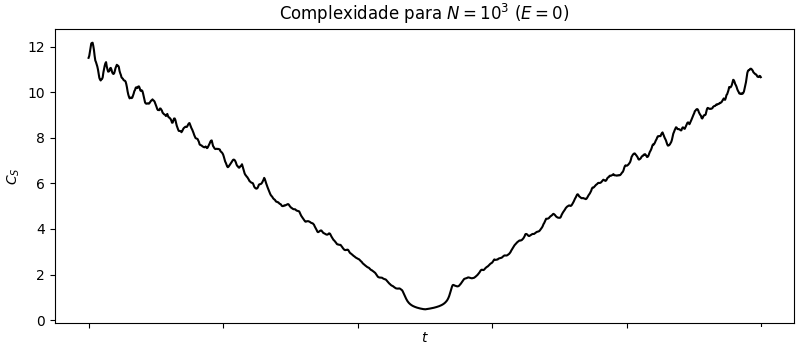
\includegraphics[width=0.5\linewidth]{tcc//img/complexidade_1000_nula.png}
%     \caption{Enter Caption}
%     \label{fig:enter-label}
% \end{figure}